% =====================================================================
% Manuscript prepared for submission to:
%   International Journal of Sports Physiology and Performance (IJSPP)
%   Human Kinetics -- Original Investigation
%
% Formatting follows IJSPP author guidelines for initial submission:
%   - Double-spaced, 12 pt, continuous line numbers
%   - Structured abstract (Purpose / Methods / Results / Conclusions)
%   - Practical Applications section
%
% This is a reframed version of grad.tex. The scientific content and all
% reported statistics are preserved; the narrative is reorganised around
% the route-geometry artifact and the multi-session profiling protocol,
% rather than around the dimensionality of the Meixner framework.
% =====================================================================
\documentclass[12pt]{article}

\usepackage[margin=1in]{geometry}
\usepackage{setspace}
\usepackage{lineno}
\usepackage{amsmath}
\usepackage{bm}
\usepackage{booktabs}
\usepackage{graphicx}
\usepackage{times}
\usepackage[hidelinks]{hyperref}

\graphicspath{{Figures/}}

\doublespacing
\linenumbers

\title{Gradient-Adjusted Cardiac Drift: Correcting the Route-Geometry
Artifact in Field-Based Aerobic Decoupling and a Multi-Session
Reliability Protocol for Individual Profiling}

\author{Hisashi Ikari\\
\small Independent Researcher\\
\small Corresponding author: hisashi@ikari.io}

\date{}

\begin{document}

\maketitle

\noindent\textbf{Manuscript type:} Original Investigation

\noindent\textbf{Running head:} Gradient-Adjusted Cardiac Drift

\noindent\textbf{Abstract word count:} 246

\noindent\textbf{Text word count:} $\sim$3{,}900 (excluding abstract, references, tables, figure legends)

\noindent\textbf{Number of tables:} 4 \qquad \textbf{Number of figures:} 3

\vspace{1em}

% =====================================================================
\section*{Abstract}
% =====================================================================
\noindent\textbf{Purpose:} The speed-based Decoupling Index (DI $=$ HR/speed)
is displayed to millions of endurance athletes by GPS-watch platforms
(e.g., TrainingPeaks, Strava) as a marker of aerobic durability, yet its
sensitivity to route terrain has never been quantified. We aimed to
(1)~quantify the route-geometry artifact in field-based DI, (2)~test
whether a regression-based Gradient-Adjusted Cardiac Drift (GACD)
correction removes it, and (3)~derive the number of sessions required
for reliable individual profiling.

\noindent\textbf{Methods:} We analysed $N = 13{,}750$ real-world workouts
from $K = 675$ users in the public FitRec (Endomondo) dataset. A
controlled simulation ($N = 5{,}000$ synthetic workouts, cardiac drift
fixed to zero, all parameters drawn from the data) established the
theoretical artifact ceiling. Route predictability of DI versus
GACD-derived metrics was assessed by group $k$-fold cross-validated
$R^2$. Reliability was quantified by intraclass correlation
(ICC(1,1)), route-matched ICC, and Spearman--Brown (SB) convergence
across aggregated sessions.

\noindent\textbf{Results:} With zero cardiac drift, route geometry alone
produced DI from 0.70 to 1.40 (cross-validated $R^2 = 0.80$). In real
data, route features predicted DI with $R^2 = 0.49$ (0.72 on hilly
terrain); after GACD correction, predictability was eliminated
($R^2 \approx 0.02$). Day-to-day (Occasion) variance dominated all
metrics (56--84\%). Gradient sensitivity from GACD reached adequate
reliability (SB $\geq 0.80$) at $\geq 5$ aggregated sessions.

\noindent\textbf{Conclusions:} Speed-based DI is heavily contaminated by
route geometry, and 42\% of routes mechanically produce DI $< 1.0$
without any cardiac drift. GACD removes this artifact, and multi-session
aggregation ($\geq 5$ sessions) yields a reliable individual durability
profile for field monitoring.

\vspace{1em}
\noindent\textbf{Keywords:} aerobic decoupling; durability; cardiac
drift; gradient correction; reliability; wearable monitoring

\clearpage

% =====================================================================
\section{Introduction}
% =====================================================================
Aerobic decoupling---the progressive rise in heart rate (HR) relative to
pace or power during prolonged exercise---is widely used as a field-based
indicator of endurance fitness.\textsuperscript{1,2} Consumer platforms
such as TrainingPeaks and Strava present the Decoupling Index (DI) to
millions of athletes and apply Friel's $<5\%$ threshold\textsuperscript{2}
to signal an adequate aerobic base. This threshold has never been
empirically validated in a peer-reviewed study, and---critically---the
metric is almost universally computed as HR/speed on consumer GPS
watches, not as the HR/power ratio assumed in the physiological
literature.\textsuperscript{3}

On variable terrain, speed is determined primarily by gradient, so
speed-based DI necessarily carries a route-geometry component. Consider a
front-loaded course: an athlete who climbs early and descends late will
record a high HR/low speed in the first half and a low HR/high speed in
the second half, mechanically producing DI $< 1.0$---the appearance of
``negative drift''---even with a perfectly stable cardiovascular system.
What has not been established is (a)~the \emph{magnitude} of this
component, (b)~whether it \emph{dominates} the physiological signal in
real-world data, and (c)~what signal \emph{remains} once it is corrected.
The most closely related large-scale work, Smyth et al.\ in 82,303
marathon runners,\textsuperscript{4} established that decoupling magnitude
and onset predict performance, but did not examine the route-geometry
artifact or the reliability of the measure for individual monitoring.

The reliability of field-based HR metrics has long been a
concern,\textsuperscript{5,6} and the IOC consensus\textsuperscript{7}
emphasises the external-load/internal-response distinction. Yet no study
has quantified how much of the variance in HR-response metrics is
attributable to the person, the route, and the transient daily state
(occasion)---the very partition that determines how many sessions a
practitioner must average before a value is trustworthy.

Recent physiological work has framed endurance ``durability'' as a
multi-dimensional construct.\textsuperscript{3,8,9} Whether such
constructs are empirically separable when operationalised with the
speed-based field metrics that athletes actually use is unknown; we treat
this dimensionality question as a secondary, exploratory analysis and
focus the present study on the measurement problem that has immediate
practical consequences.

\noindent\textbf{Aims.} This study addresses three questions:
\begin{itemize}
  \item[\textbf{A1}] How large is the route-geometry artifact in
  speed-based DI, and does it dominate the physiological signal?
  \item[\textbf{A2}] Does a within-workout Gradient-Adjusted Cardiac
  Drift (GACD) regression remove the artifact and isolate the
  physiological signal?
  \item[\textbf{A3}] How many sessions must be aggregated for a
  GACD-derived metric to reach adequate individual reliability
  (Spearman--Brown $\geq 0.80$)?
\end{itemize}

% =====================================================================
\section{Methods}
% =====================================================================
\subsection{Data and filtering}
The publicly available FitRec dataset,\textsuperscript{10} comprising
253,020 GPS-tracked Endomondo workouts, was used. Each record contains
irregularly time-stamped arrays of HR (optical wrist sensor, bpm), speed
(GPS-derived, km$\cdot$h$^{-1}$), altitude (m), and geographic
coordinates. Where the recorded speed array was missing or shorter than
10 points, speed was derived from GPS coordinates via the Haversine
formula (values $>150$~km$\cdot$h$^{-1}$ excluded as outliers). The
cohort is 94.6\% male; age, body mass, and training history are
unavailable.

A four-step inclusion pipeline was applied: (1)~HR, altitude, and speed
arrays each required $\geq 30$ finite points (missing values linearly
interpolated); (2)~total duration $>90$~min, ensuring sufficient time for
cardiac drift to manifest;\textsuperscript{1} (3)~altitude range
$>200$~m, ensuring sufficient gradient variation to confound DI (median
retained $= 349$~m); for suspected loop routes ($>80\%$ overlap) the
start-to-end altitude deviation was required to be $<50$~m to control
barometric drift; (4)~each temporal half required $\geq 6$ points with
speed $>0.5$~km$\cdot$h$^{-1}$. This yielded $N = 13{,}750$ workouts from
$K = 675$ users for Study~1 (cycling 61.8\%, running 16.9\%, mountain
biking 16.7\%, other 4.6\%; median duration 181~min). Analyses requiring
$\geq 5$ repeated workouts per user (Studies~2--3) used a high-engagement
subset of $N = 2{,}343$ workouts from $K = 314$ users (cycling 83.9\%;
median duration 208~min).

\subsection{Speed-based indices}
Three speed-based indices were computed per workout. The
\textbf{Decoupling Index (DI)} is the second-to-first-half ratio of
HR/speed; DI $>1$ indicates positive drift. The \textbf{Fading Index
(FI)} is the gradient-binned ratio of second-to-first-half speed
(fatigability), averaged over five gradient bins populated in both
halves. The \textbf{Resilience Index (RI)} is the ratio of speed on the
last versus first sustained climb ($>50$~m vertical gain). Person-level
medians were used for aggregation because of heavy-tailed distributions
(e.g., FI kurtosis $= 590$). Full equations are given in the
Supplementary Material.

\subsection{Gradient-Adjusted Cardiac Drift (GACD) regression}
For each workout with $\geq 20$ valid points, HR was modelled at
consecutive midpoints as a linear function of gradient ($g$, \%; clipped
to $\pm 50\%$), speed ($v$, m$\cdot$s$^{-1}$), and time ($t$, min):
\begin{equation}
  \mathrm{HR}_i = \beta_0 + \beta_{\mathrm{grad}}\, g_i
  + \beta_{\mathrm{speed}}\, v_i + \beta_{\mathrm{time}}\, t_i
  + \varepsilon_i .
  \label{eq:gacd}
\end{equation}
$\beta_{\mathrm{time}}$ (bpm$\cdot$min$^{-1}$) captures the
within-session HR drift after removing terrain and pace confounds;
$\beta_{\mathrm{grad}}$ (bpm$\cdot$\%$^{-1}$) and $\beta_{\mathrm{speed}}$
are interpreted as route-corrected, submaximal fitness-profiling
coefficients. Multicollinearity was minimal (median VIF: gradient 2.01,
speed 2.09, time 1.07; 99.8\% of sessions VIF $<10$).\textsuperscript{11}

\subsection{Study 1 --- Quantifying and correcting the artifact (A1, A2)}
\textbf{Route predictability.} Thirteen route features (total
ascent/descent, altitude range, max/min altitude, gradient mean/SD,
climb/descent/flat fractions, ascent-front and descent-front ratios,
duration) were used to predict each metric via RidgeCV
($\alpha \in \{0.01,0.1,1,10,100\}$) and gradient-boosted trees.
Generalisation was assessed by group $k$-fold cross-validated $R^2$
($k = \min(5, K_{\mathrm{valid}})$; all workouts of a user in the same
fold). For GACD the target was the within-person deviation, isolating
route effects from person means.

\textbf{Controlled simulation.} $N = 5{,}000$ synthetic workouts were
generated with cardiac drift fixed to \emph{exactly zero}; all
distributional parameters (route-type proportions, gradient asymmetry,
per-workout HR and speed parameters) were drawn from the FitRec data.
Any deviation of simulated DI from 1.0 therefore arises purely from
gradient asymmetry, establishing the theoretical ceiling of the
artifact.

\textbf{Estimated-power comparison.} As an alternative correction, DI was
recomputed replacing speed with estimated metabolic power
$P = v \cdot C_w(g)$, where $C_w(g)$ is the Minetti walking cost
polynomial.\textsuperscript{12}

\subsection{Study 2 --- Variance structure and reliability protocol (A3)}
For users with $\geq 5$ workouts, one-way random-effects
ICC(1,1)\textsuperscript{13} quantified between-person (Person) variance.
Within-person deviations were predicted from route features (RidgeCV,
group $k$-fold CV) to estimate the Route share; the residual defined the
Occasion share. Uncertainty was estimated by user-level bootstrap
($B = 500$). A \textbf{route-matched} analysis paired each user's
workouts within $\pm 20\%$ of altitude range and total ascent
($n = 451$ pairs, 95 users) to provide an upper-bound Person estimate.
\textbf{Split-half reliability} (Spearman--Brown corrected) was computed
for users with $\geq 10$ workouts, and a \textbf{convergence analysis}
(for $k = 2,\dots,10$ randomly sampled sessions) identified the minimum
$k$ for SB $\geq 0.80$.

\subsection{Secondary analyses}
Construct dimensionality was examined by PCA with parallel
analysis\textsuperscript{14} on person-level medians, and by pairwise
bootstrap correlations ($B = 2{,}000$) among DI, FI, and RI. An
exploratory descent-placement analysis (between- and within-person,
FDR-corrected\textsuperscript{15}) tested whether the temporal position
of descent relates to cardiac drift.

\subsection{Sensitivity analysis: temporal autocorrelation}
Point-level GPS data violate the OLS independence assumption. On a random
subsample ($N = 300$; median 499 points), we computed Durbin--Watson (DW)
statistics, the autocorrelation function of GACD residuals, and
Newey--West HAC standard errors. Because the study's conclusions rest on
workout-level and person-level aggregates rather than point-level
inference, autocorrelation affects per-workout $R^2$ and standard errors
but not the OLS point estimates on which profiling depends.

\subsection{Software}
Python 3.12 (NumPy 1.26, SciPy 1.13, pandas 2.2, scikit-learn 1.5; seed
42). Code and reproducibility scripts:
\url{https://github.com/ikari12/GRAD}.

% =====================================================================
\section{Results}
% =====================================================================
\subsection{A1: The route-geometry artifact dominates speed-based DI}
The mean DI across all workouts was 0.92 (Table~\ref{tab:descriptive}),
indicating that HR/speed was, on average, \emph{lower} in the second
half---an apparent negative cardiac drift. This counterintuitive result
is explained by route geometry. Classifying routes by the fraction of
climbing in the first half (ascent-front) revealed three distinct DI
distributions: front-climb routes (ascent-front $>0.6$; 42.4\%) had a
median DI of 0.770 (fast descent in the second half mechanically
depresses DI); symmetric routes yielded a median of 0.978; and back-climb
routes (10.1\%) a median of 1.157 (Supplementary Figure~S1).

The controlled simulation confirmed the mechanism directly: with cardiac
drift fixed to zero, route geometry alone produced DI values from 0.70 to
1.40, with cross-validated $R^2 = 0.80$
(Figure~\ref{fig:simulation}A)---the theoretical ceiling of the artifact.
In real data, route features predicted naive DI with cross-validated
$R^2 = 0.49$ (all routes) and $0.72$ (hilly subset, $\Delta a > 400$~m).
Thus a majority of the variance in the metric that millions of athletes
interpret physiologically is, in fact, terrain.

\begin{table}[t]
\centering
\caption{Descriptive statistics of the speed-based durability metrics
($N = 13{,}750$).}
\label{tab:descriptive}
\begin{tabular}{@{}lccccc@{}}
\toprule
Metric & $N$ & Mean & SD & Median & IQR [Q1, Q3] \\
\midrule
DI & 13,549 & 0.92 & 0.26 & 0.92 & [0.78, 1.04] \\
FI & 13,742 & 1.06 & 0.23 & 1.04 & [0.95, 1.14] \\
RI & 10,032 & 0.99 & 0.29 & 0.95 & [0.80, 1.13] \\
\bottomrule
\end{tabular}
\end{table}

\begin{figure}[t]
\centering
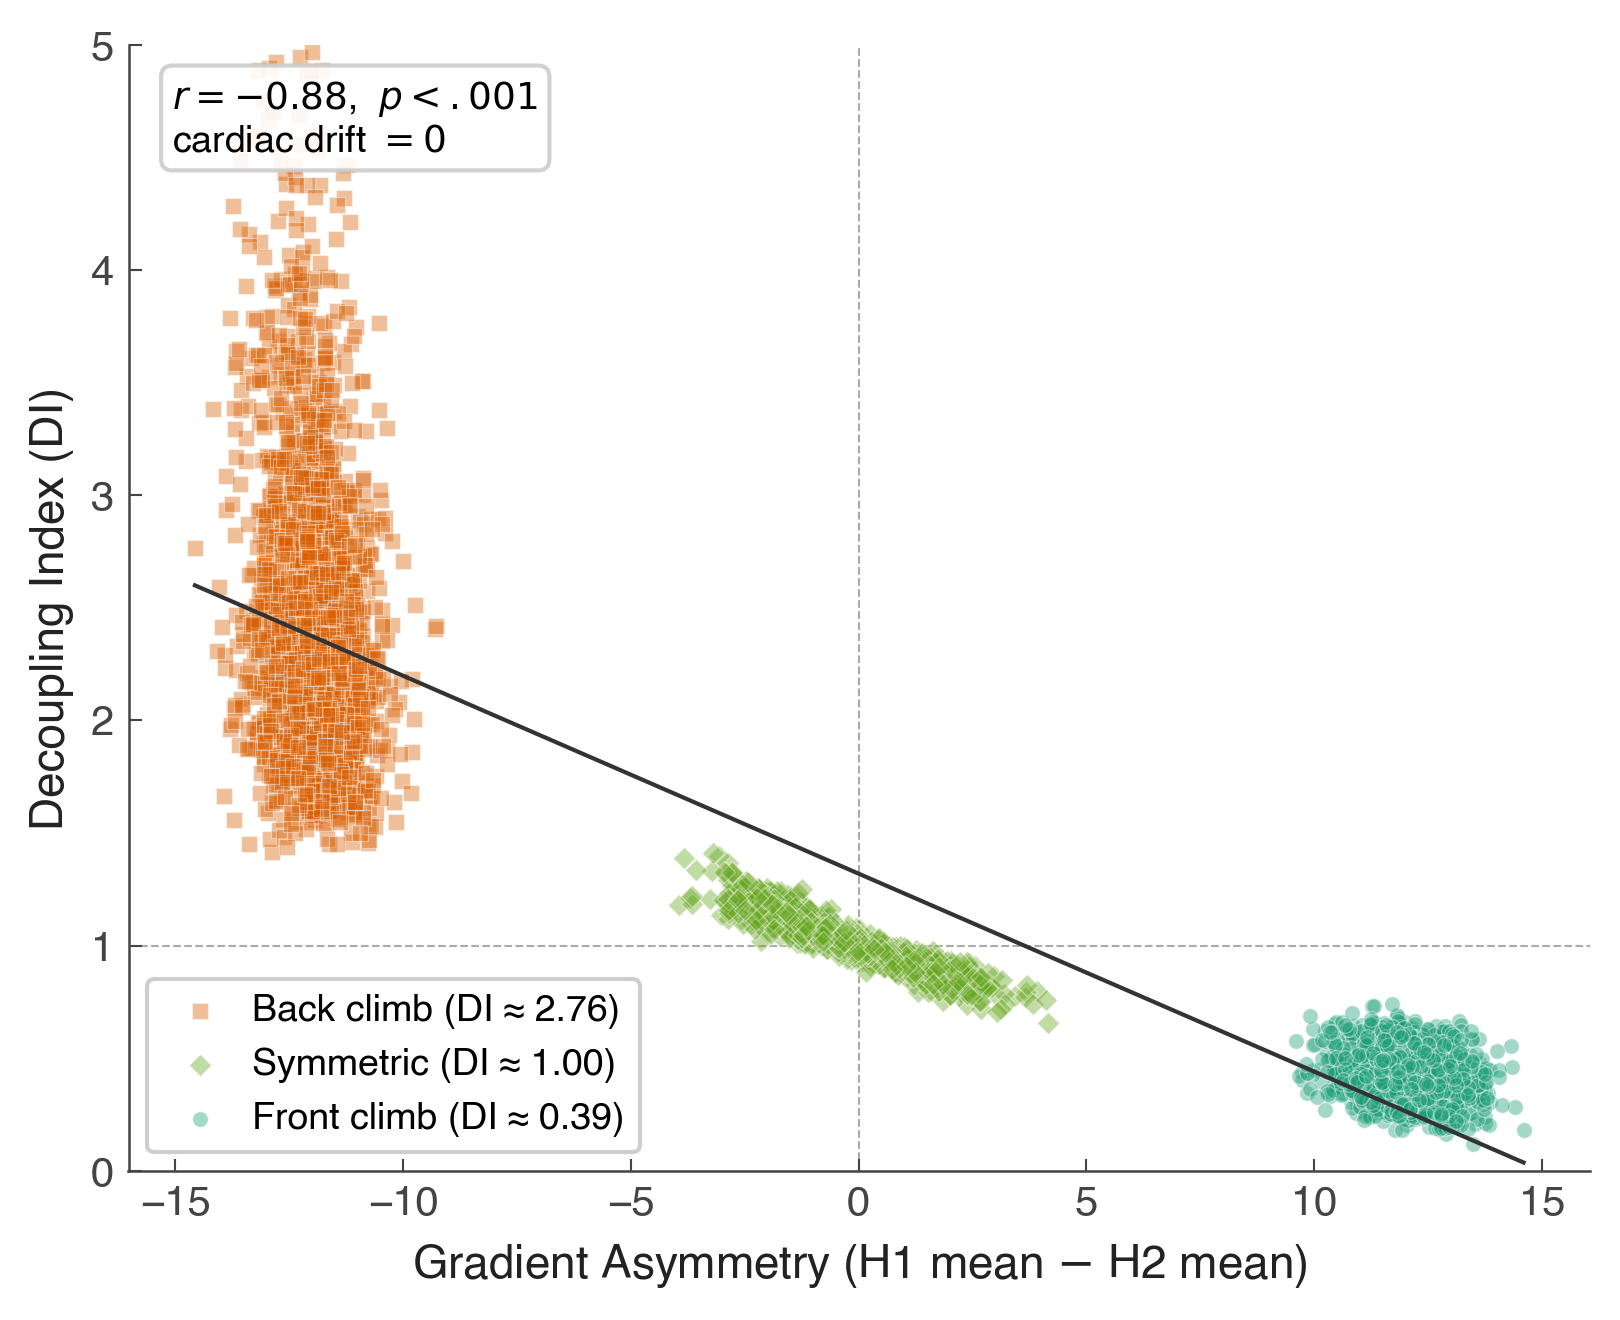
\includegraphics[width=\linewidth]{fig1_simulation.png}
\caption{Quantifying the route-geometry artifact. (A)~With cardiac drift
fixed to zero, route geometry alone produces DI values between 0.70 and
1.40. (B)~Cross-validated route predictability ($R^2$) of naive DI versus
GACD-corrected metrics.}
\label{fig:simulation}
\end{figure}

\subsection{A2: GACD removes the artifact and isolates the signal}
Applying the GACD regression (Eq.~\ref{eq:gacd}) eliminated route
predictability: within-person GACD deviations were essentially
unpredictable from route features (cross-validated $R^2 \approx +0.02$;
Figure~\ref{fig:simulation}B), reducing the artifact from the empirical
$0.49$ and the theoretical $0.80$ to near zero. This confirms that a
simple, per-session linear correction is sufficient to separate the
physiological drift signal from terrain.

Replacing speed with estimated metabolic power did \emph{not} achieve
this. DI/estimated-power showed a route dependency of comparable
magnitude but opposite sign ($r = -0.46$ vs.\ $+0.49$ for DI/speed;
cross-validated $R^2 = 0.20$), worsening on hilly terrain ($r = -0.56$,
$R^2 = 0.31$). The reversal arises because the Minetti cost function
drops on descents (minimum $\approx 0.94$~J$\cdot$kg$^{-1}\cdot$m$^{-1}$
near $-15.4\%$ vs.\ 2.5 at 0\%), inflating the denominator on
early-descent routes; the walking-derived cost function is also
mismatched to a cycling-dominated dataset. The data-driven GACD
regression is therefore the preferred correction, because it learns the
modality-specific submaximal relationship directly from each workout.

\subsection{A3: Occasion dominates variance; $\geq 5$ sessions restore
reliability}
Day-to-day Occasion variance dominated every metric (56--84\%;
Table~\ref{tab:main}), which explains why single-session field values are
unreliable. Crucially, this within-person variability is
\emph{manageable} by aggregation. Route-matched analysis showed that a
substantial part of the apparent Occasion variance is actually
route-related and controllable: holding route approximately constant
raised Person estimates for GACD ($0.22 \rightarrow 0.47$), gradient
sensitivity ($0.38 \rightarrow 0.56$), and speed sensitivity
($0.44 \rightarrow 0.74$)---18--31 percentage points.

\begin{table}[t]
\centering
\caption{Variance structure and reliability on hilly terrain
($\Delta a > 400$~m). Route-corrected coefficients are derived from
Eq.~\ref{eq:gacd}.}
\label{tab:main}
\begin{tabular}{@{}lcccc@{}}
\toprule
Metric & ICC(1,1) & Route-matched ICC & SB ($k{=}5$) & Route CV $R^2$ \\
\midrule
DI & 0.16 & 0.45 & 0.62 & 0.49 \\
GACD ($\beta_{\mathrm{time}}$) & 0.22 & 0.47 & 0.85 & $+0.02$ \\
Gradient sensitivity & 0.38 & \textbf{0.56} & \textbf{0.91} & $+0.04$ \\
Speed sensitivity & \textbf{0.44} & \textbf{0.59} & \textbf{0.93} & $-0.09$ \\
\bottomrule
\end{tabular}
\end{table}

The convergence analysis translated this into a concrete protocol
(Figure~\ref{fig:convergence}): gradient sensitivity crossed the
SB $= 0.80$ threshold at $k = 5$ sessions (SB$_5 = 0.80$,
SB$_{10} = 0.88$) and speed sensitivity at $k = 3$ (SB$_3 = 0.81$),
whereas naive DI never reached 0.80 by $k = 10$ (SB$_{10} = 0.71$).
Gradient sensitivity also showed the most balanced profile overall: the
only positive route CV $R^2$ ($+0.047$) and the strongest correlation
with an external criterion (user-level median speed, $r = +0.36$;
Table~\ref{tab:comparison}). The marked ICC--SB discrepancy (DI: 0.16 vs.\
0.62; gradient sensitivity: 0.38 vs.\ 0.91) indicates that rank-order
consistency across sessions is preserved even when absolute values
fluctuate---so within-person \emph{trends} are interpretable once
$\geq 5$ sessions are averaged.

\begin{figure}[t]
\centering
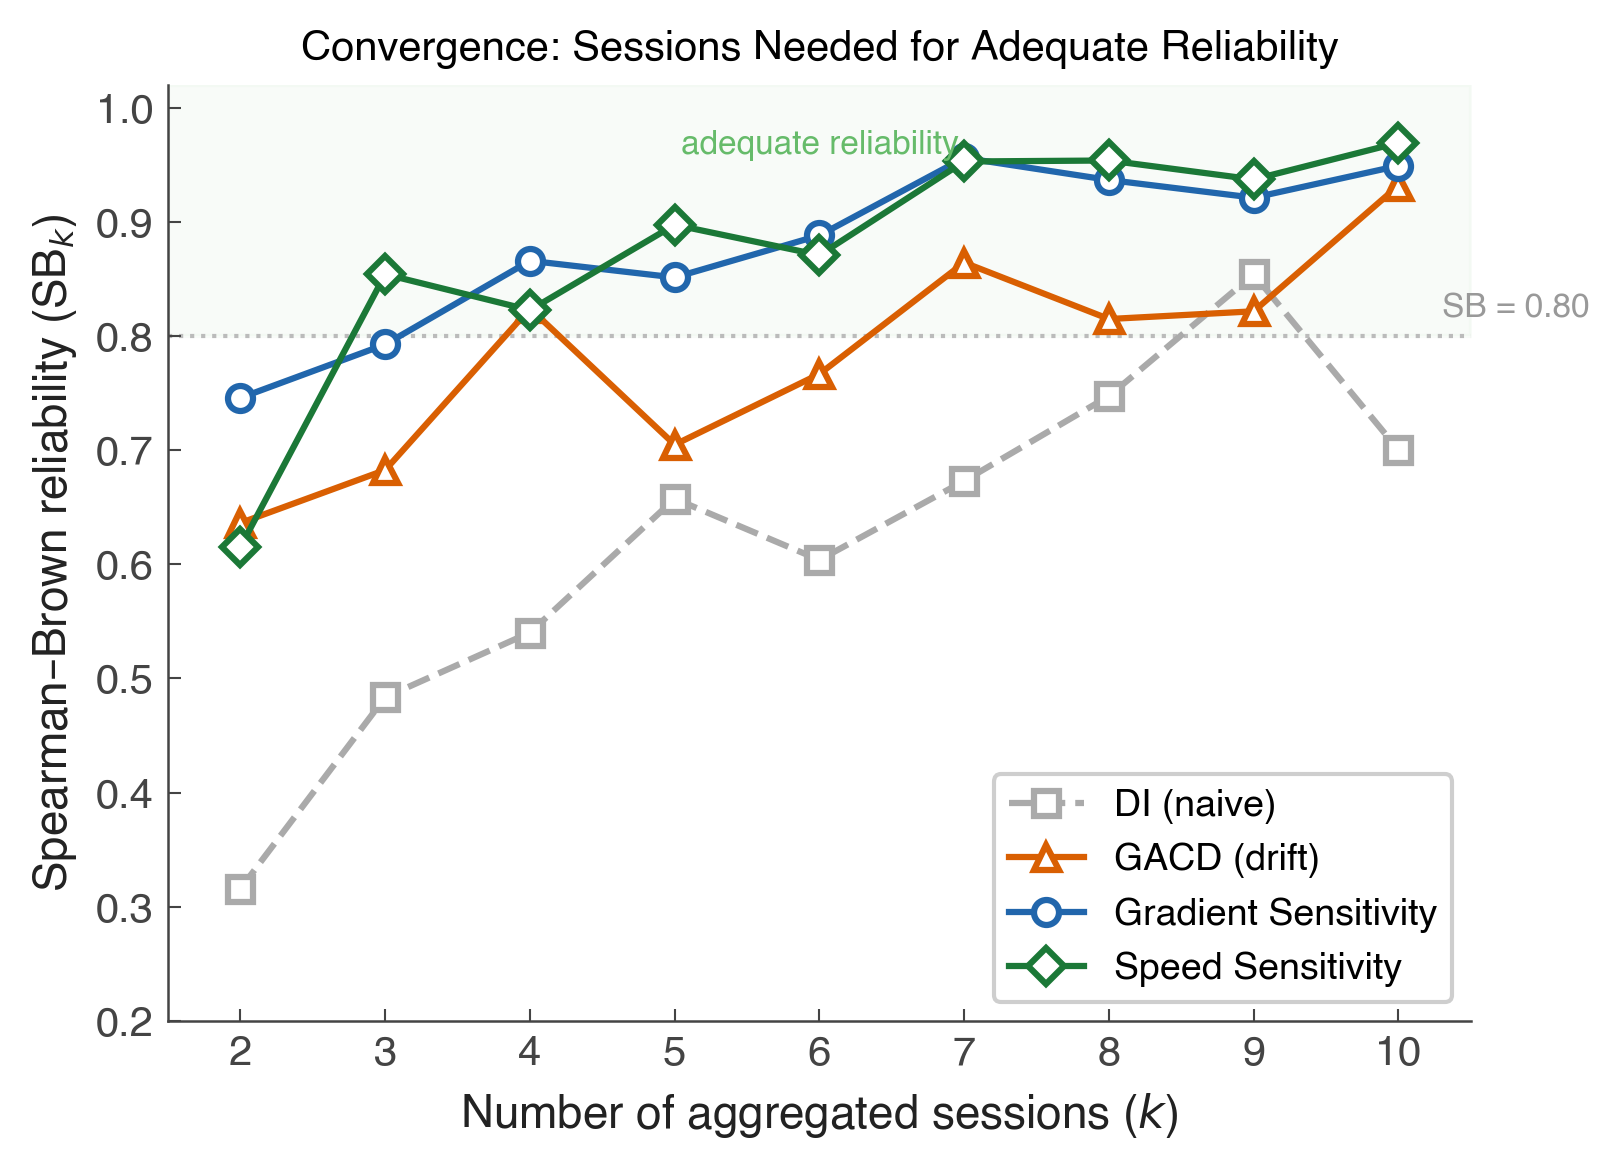
\includegraphics[width=0.9\linewidth]{fig3_convergence.png}
\caption{Variance decomposition and multi-session reliability.
(A)~Variance partitioning for gradient sensitivity. (B)~Spearman--Brown
reliability as a function of the number of aggregated sessions ($k$).
Gradient sensitivity crosses SB $= 0.80$ at $k = 5$; DI and GACD do not
reach 0.80 by $k = 10$.}
\label{fig:convergence}
\end{figure}

\begin{table}[t]
\centering
\caption{Head-to-head comparison of DI and the proposed GACD-derived
profiling metrics on hilly terrain ($\Delta a > 400$~m). Route CV $R^2$
near zero indicates successful removal of the geometric artifact.}
\label{tab:comparison}
\begin{tabular}{@{}lccc@{}}
\toprule
 & DI & Gradient sensitivity & Speed sensitivity \\
\midrule
Unadjusted ICC & 0.16 & 0.38 & 0.44 \\
Route-matched ICC & 0.47 & \textbf{0.56} & \textbf{0.59} \\
SB reliability ($k{=}5$) & 0.55 & \textbf{0.80} & \textbf{0.90} \\
Route CV $R^2$ & $+0.006$ & \textbf{$+0.047$} & $-0.090$ \\
Speed correlation ($r$) & $-0.15$ & \textbf{$+0.36$} & $+0.28$ \\
\bottomrule
\end{tabular}
\end{table}

\subsection{Secondary: dimensionality and descent placement}
DI and FI were strongly negatively correlated ($r = -0.60$, 95\% CI
$[-0.69, -0.49]$), and consistently so across cycling ($-0.62$), running
($-0.50$), and mountain biking ($-0.58$), indicating that both indices
capture the same gradient-response coupling that GACD removes. PCA
retained one factor; the second eigenvalue (1.005) fell marginally below
the parallel-analysis threshold (1.031) by only 0.026 units, providing
\emph{fragile} support for a two-construct organisation (DI/FI redundant;
RI apparently independent but unreliable, ICC $= 0.10$). This
dimensionality result should be treated as exploratory. Exploratory
analysis further linked descent \emph{placement} (front-loaded) to
greater cardiac drift between persons ($r = +0.16$, $p_{\mathrm{FDR}} <
.001$, moderated by steepness and absent in mountain biking), with only
modest within-person support ($\bar r = +0.082$); the effect is
suggestive but not confirmatory.

\subsection{Robustness}
The DI--FI redundancy was stable across 25 combinations of duration
(60--120~min) and altitude-range (100--300~m) thresholds ($\bar r =
-0.60$, SD $= 0.02$). The temporal-autocorrelation sensitivity analysis
confirmed strong point-level autocorrelation (median DW $= 0.355$; lag-1
ACF $= 0.803$; Supplementary Figures~S2a--b), inflating per-workout $R^2$
(median 0.82) and roughly doubling standard errors (Newey--West vs.\ OLS
$\approx 2\times$); however, OLS point estimates remain unbiased, and the
core cross-validated, PCA, ICC, and convergence results operate on
workout- or person-level aggregates and are unaffected.

% =====================================================================
\section{Discussion}
% =====================================================================
This study delivers three practically consequential findings. First, the
speed-based DI that millions of athletes rely on is dominated by route
geometry: with cardiac drift fixed to zero, terrain alone explains 80\%
of DI variance, and in real data it explains roughly half. A direct
corollary is that 42\% of routes---front-climb profiles---mechanically
produce DI $< 1.0$ regardless of fitness. Athletes on hilly terrain who
see DI $< 1.0$ on their GPS platform are therefore likely
mis-interpreting a geometric artifact as evidence of an excellent aerobic
base. This is, to our knowledge, the first quantification of a systematic
bias in a metric that is already in daily use at population scale.

Second, the artifact is correctable with a simple per-session linear
model. GACD reduces route predictability from 0.49 (empirical) and 0.80
(theoretical ceiling) to $\approx 0.02$, isolating the physiological
drift signal. Notably, the seemingly more principled alternative---
converting speed to estimated metabolic power via a published cost
function---\emph{over}-corrects and reverses the bias, because a rigid,
walking-derived cost function cannot adapt to mixed-modality field data.
The advantage of GACD is precisely that it learns each individual's
submaximal HR--gradient--speed relationship from the signal itself,
making it a general tool for isolating cardiac drift from any
terrain-confounded ratio. Unlike commercial Grade-Adjusted Pace, which
corrects pace for gradient but ignores time-dependent drift, GACD
addresses both simultaneously.

Third, and most important for practitioners, the variance structure
dictates the measurement protocol. Occasion accounts for 56--84\% of
variance---not a nuisance to be minimised, but the central quantitative
argument for aggregation. Controlled laboratory settings suppress
day-to-day variation by design, creating the illusion that one session
suffices; the ecological scale here (253,020 real-world workouts) exposes
the true session-to-session fluctuation practitioners face. Gradient
sensitivity emerges as the best single candidate: it is the only metric
whose route-corrected within-person deviations remain positively
predictable, it correlates most strongly with external speed, and it
reaches SB $\geq 0.80$ at $\geq 5$ aggregated sessions. The preserved
rank-order consistency (large ICC--SB gap) further means that
longitudinal \emph{trends} across training blocks are interpretable even
when individual sessions vary.

\textbf{A dual-profiling framework.} The three GACD coefficients play
distinct roles: $\beta_{\mathrm{time}}$ indexes within-session drift
(durability), whereas $\beta_{\mathrm{grad}}$ and $\beta_{\mathrm{speed}}$
are route-corrected fitness-capacity profiles. We note that
$\beta_{\mathrm{time}}$ is related to, but distinct from, the
between-session durability construct of Maunder et al.,\textsuperscript{8}
which concerns fatigue-induced shifts in the power--duration
relationship.

\textbf{Limitations.} (1)~DI here is HR/speed, not HR/power; HR/speed is a
weaker proxy for cardiac efficiency in cycling---where power, drag, and
rolling resistance intervene---than in running. GACD absorbs terrain
variance but not residual aerodynamic/mechanical confounds. (2)~The
dataset is cycling-dominated (61.8\% overall; 83.9\% of the
high-engagement subset), and the running subsample in that subset is too
small ($3$ users with $\geq 5$ sessions) for stable estimation; the
$\geq 5$-session recommendation should be considered primarily
cycling-specific pending running-specific validation. (3)~Secondary data
with uncontrolled, wrist-optical HR sensors of variable
accuracy;\textsuperscript{6} sensor noise likely inflates Occasion
variance. (4)~No gold-standard criterion (VO$_2$max, power). (5)~94.6\%
male, limiting generalisability, particularly given documented sex
differences in cardiovascular drift. (6)~Point-level temporal
autocorrelation means per-workout inference (not point estimates) is
unreliable; GLS was not applied. (7)~The two-construct dimensionality
conclusion rests on a fragile 0.026-unit eigenvalue margin and is
exploratory. (8)~RI (ICC $= 0.10$) is unreliable and its apparent
independence may reflect noise. (9)~Descent-placement and other
exploratory findings were not pre-registered.

% =====================================================================
\section{Practical Applications}
% =====================================================================
\begin{itemize}
  \item \textbf{Do not interpret raw DI on hilly terrain.} A DI $< 1.0$
  on a front-loaded (climb-early, descend-late) course is most likely a
  route-geometry artifact, not evidence of superior aerobic fitness. On
  variable terrain the Friel $<5\%$ rule of thumb should not be applied
  to uncorrected, speed-based DI.
  \item \textbf{Apply GACD before interpreting drift.} Fitting a simple
  per-session linear model of HR on gradient, speed, and time removes the
  terrain confound and isolates the physiological drift
  ($\beta_{\mathrm{time}}$). This is more robust than converting speed to
  an estimated-power cost function, which over-corrects on descents.
  \item \textbf{Aggregate at least five sessions.} Because day-to-day
  variation dominates single sessions (56--84\%), practitioners should
  average $\geq 5$ sessions of gradient sensitivity (or $\geq 3$ of speed
  sensitivity) before drawing conclusions about an athlete's durability
  profile.
  \item \textbf{Track trends, not single values.} Rank-order stability is
  preserved across sessions, so within-athlete trends across training
  blocks are interpretable even when absolute session values fluctuate.
  \item \textbf{Use sport-specific baselines.} Gradient sensitivity
  differs markedly across modalities (cycling $+2.11$, MTB $+1.17$,
  running $+0.47$ bpm$\cdot$\%$^{-1}$), so comparisons should be made
  within sport.
\end{itemize}

% =====================================================================
\section{Conclusions}
% =====================================================================
Speed-based aerobic decoupling, as displayed to millions of athletes, is
heavily contaminated by route geometry---up to 80\% of its variance under
controlled conditions and roughly half in the field---so that a large
fraction of hilly-route DI values are geometric artifacts rather than
physiological signal. A simple within-session Gradient-Adjusted Cardiac
Drift regression removes this artifact ($R^2$ predictability
$0.49/0.80 \rightarrow 0.02$) and yields route-corrected profiling
coefficients. Because transient day-to-day state dominates single-session
variance, reliable individual profiling requires multi-session
aggregation: gradient sensitivity reaches adequate reliability at
$\geq 5$ sessions. Together these provide an actionable, field-deployable
protocol for durability monitoring on variable terrain.

% =====================================================================
\section*{Acknowledgements}
% =====================================================================
The author thanks the developers and contributors of the FitRec dataset
and the Endomondo community for making the telemetry data available for
research. No external funding was received. The author declares no
competing interests. This study is a secondary analysis of the publicly
available, de-identified FitRec dataset\textsuperscript{10} and did not
require institutional ethics review.

% =====================================================================
\section*{References}
% =====================================================================
\begin{enumerate}
  \item Coyle EF, Gonzalez-Alonso J. Cardiovascular drift during
  prolonged exercise: new perspectives. \textit{Exerc Sport Sci Rev}.
  2001;29(2):88--92.
  \item Friel J. \textit{The Cyclist's Training Bible}. VeloPress; 2009.
  \item Meixner BJ, Joyner MJ, Sperlich B. Durability, fatigability,
  repeatability, and resilience in endurance sports: definitions,
  distinctions, and implications. \textit{J Appl Physiol}.
  2025;139(6):1703--1709. doi:10.1152/japplphysiol.00343.2025
  \item Smyth B, et al. Cardiovascular drift and marathon performance.
  \textit{Sports Med}. 2022;52(9):2283--2295.
  \item Hopkins WG. Measures of reliability in sports medicine and
  science. \textit{Sports Med}. 2000;30(1):1--15.
  \item Halson SL. Monitoring training load to understand fatigue in
  athletes. \textit{Sports Med}. 2014;44(2):139--147.
  \item Bourdon PC, et al. Monitoring athlete training loads: consensus
  statement. \textit{Int J Sports Physiol Perform}.
  2017;12(s2):S2-161--S2-170.
  \item Maunder E, et al. The importance of physiological durability to
  endurance performance. \textit{Sports Med}. 2021;51(8):1619--1628.
  \item Jones AM. The fourth dimension: physiological resilience as an
  independent determinant of endurance exercise performance.
  \textit{J Physiol}. 2024;602(17):4113--4128. doi:10.1113/JP284205
  \item Ni J, Muhlstein L, McAuley J. Modeling heart rate and simulating
  workouts in size-varying datasets. \textit{The World Wide Web
  Conference (WWW '19)}. 2019:1343--1353.
  \item Hair JF, et al. \textit{Multivariate Data Analysis}. Pearson;
  2010.
  \item Minetti AE, et al. Energy cost of walking and running at extreme
  uphill and downhill slopes. \textit{J Appl Physiol}.
  2002;93(3):1039--1046.
  \item Shrout PE, Fleiss JL. Intraclass correlations: uses in assessing
  rater reliability. \textit{Psychol Bull}. 1979;86(2):420--428.
  \item Horn JL. A rationale and test for the number of factors in factor
  analysis. \textit{Psychometrika}. 1965;30(2):179--185.
  \item Benjamini Y, Hochberg Y. Controlling the false discovery rate: a
  practical and powerful approach to multiple testing. \textit{J R Stat
  Soc B}. 1995;57(1):289--300.
\end{enumerate}

\end{document}
